\documentclass{beamer}
\usepackage{etex}
\usepackage[beamer]{mydefs}
\usepackage{todonotes}
\usepackage{xspace}
\usepackage{listings}
\usepackage{tikz,pgfplots}
\usepackage{alltt}

%%%

\title[\cclj]{Exploratory Programming for Formal Concept Analysis}
\subtitle{An Introduction to \cclj}
\author{Daniel Borchmann}
\institute{TU Dresden}

%%%

\usetheme{CambridgeUS}

\newcommand{\cclj}{\texttt{conexp-clj}\xspace}

\lstdefinelanguage{Clojure}
{ alsoletter={:,-,?},
  basicstyle=\ttfamily,
  frame=none,
  language=Lisp,
  basewidth=0.5em,
  mathescape=true,
  texcl=true,
  commentstyle=\rm,
  numbers=none,
  classoffset=0,
  morekeywords={find-doc,doc,+,defn,make-context,def,fn,filter,odd?},
  keywordstyle=\color{blue},
}
\lstset{language=Clojure}

\setbeamercolor{block title}{bg=lightgray,fg=darkred!80!gray}

\newenvironment{code}[1]{\begin{block}{Code\ifx#1\empty\else~(#1)\fi}\prompt}{\end{block}}
\newcommand{\prompt}{\texttt{\textcolor{gray}{user=>}}}
\newcommand{\codeinput}[1]{\parbox[t]{0.8\linewidth}{\ifx#1\empty\else\lstinline{#1}\fi}\\}
\newcommand{\codeoutput}[1]{\textit{\texttt{#1}}\\\prompt}
\newcommand{\codeio}[2]{\onslide<+->\codeinput{#1}\onslide<+->\codeoutput{#2}}

%%%

\begin{document}

\begin{frame}
  \maketitle

  \centerline{%
    \footnotesize%
    \url{http://www.math.tu-dresden.de/~borch/conexp-clj/icfca2013-tutorial.html}}
\end{frame}

\section{Motivation}

\subsection{Why another FCA Tool?}

\begin{frame}

  \onslide<+->

  \begin{block}{Main Question}
    Why another FCA tool? \onslide<+->Many tools which can do things fast and well!
  \end{block}

  \onslide<+->

  \begin{block}{The ``Problem''}
    \begin{itemize}
    \item<+-> But what if you want to do something else?
    \item<+-> What if you want to process your results further on?
    \item<+-> What if you want to do something from which you are \emph{not completely
        sure of}?
    \end{itemize}
  \end{block}

  \onslide<+->

  \begin{block}{Solution}
    \begin{itemize}
    \item Need flexible ``FCA scripting''
    \item<+-> Hard to achieve with available tools
    \item<+-> \cclj!
    \end{itemize}
  \end{block}

\end{frame}

\subsection{Goods and Bads}

\begin{frame}

  \onslide<+->

  \begin{block}{What \cclj is good for}
    \begin{itemize}
    \item<+-> flexible tool to try out new ideas in FCA
    \item<+-> suitable for \emph{exploratory programming}, \ie trying out new algorithms
      to see if they are correct and how they behave
    \item<+-> compute non-trivial examples (pedagogical or otherwise)
    \item<+-> \emph{FCA scripting}
    \end{itemize}
  \end{block}

  \onslide<+->

  \begin{block}{What \cclj is \emph{not} good for}
    \begin{itemize}
    \item<+-> High performance computations
    \item<+-> Data-intense computations
    \item<+-> GUI enthusiasts
    \end{itemize}
  \end{block}
\end{frame}

\subsection{Main Features}

\begin{frame}

  \onslide<+->
  
  \begin{block}{Main Features of \cclj (Overview)}
    \begin{itemize}
    \item basic operations on formal contexts
    \item relational algebra with formal contexts
    \item transparent IO for formal and many-valued contexts
    \item scaling for many-valued contexts
    \item implicational theory and basic attribute exploration
    \item computing Luxenburger-bases and iceberg concept sets
    \item lattice layouts and lattice IO (some...)
    \item a bit of fuzzy-FCA
    \item interface for Java
    \item interface for sage
    \end{itemize}
  \end{block}
\end{frame}

% Use Cases?

\section{Basic Principles}

\subsection{Design Principles}

\begin{frame}

  \onslide<+->

  \begin{block}{Implementation}
    \begin{itemize}
    \item<+-> implemented in Clojure, a Lisp dialect running on the JVM
    \item<+-> highly portable (JVM)
    \item<+-> highly flexible (Lisp)
    \item<+-> transparent access to all Java functionality
    \item<+-> compiled
    \end{itemize}
  \end{block}
\end{frame}

\subsection{Installing and Running}

\begin{frame}
  \onslide<+->

  \begin{block}{Prerequisites}
    \begin{itemize}
    \item<+-> Java 1.6 or higher (JRE sufficient)
    \end{itemize}
  \end{block}

  \onslide<+->
  \begin{block}{Download and Installation}
    \begin{itemize}
    \item<+-> Go to \cclj's website: \url{http://github.com/exot/conexp-clj}
    \item<+-> Move to \emph{How to Run}
    \item<+-> Download one of the .zip files and unpack them where you want
    \end{itemize}
  \end{block}

  \onslide<+->
  \begin{block}{Running}
    \begin{itemize}
    \item<+-> Run \texttt{./bin/conexp-clj} for a simple (yet sufficient!) command-line
      interface
    \item<+-> Run \texttt{./bin/conexp-clj ---gui} for a ``convenient'' (but mostly broken)
      graphical user interface %? why ---?
    \end{itemize}
  \end{block}
\end{frame}

\subsection{Principle Workflow}

\begin{frame}
  \onslide<+->
  \begin{code}{}
    \onslide<+->
    \codeinput{1}
    \onslide<+->
    \codeoutput{1}
    \codeio{(+ 1 2)}{3}
    \codeio{(make-context \#\{1 2 3\} \#\{0 1 2\} <=)}{\ \ |0 1 2 \\
      ---+-------\\
      1 |.\ x x \\
      2 |.\ .\ x \\
      3 |.\ .\ .
    }
    \codeio{(javax.swing.JOptionPane/showMessageDialog nil "Wow!")}{nil}
  \end{code}
\end{frame}

\subsection{An Example}

\begin{frame}
  \onslide<+->
  \begin{Example}
    \onslide<+->
    live!
  \end{Example}
\end{frame}

\section{Outlook}

\subsection{More Concepts}

\begin{frame}
  \onslide<+->
  \begin{code}{Functions}
    \codeio{(defn f [x] (+ x 3))}{\#'user/f}
    \codeio{(f 5)}{8}
    \onslide<+->
    \codeinput{(def f (fn [x] (+ x 3)))}
  \end{code}
  \onslide<+->
  \begin{code}{Functional Programming}
    \codeio{(reduce + [1 2 3 4 5])}{15}
    \codeio{(reduce * (range 1 10))}{362880}
    \codeio{(map f [4 5 6])}{(7 8 9)}
    \codeio{(filter odd? [1 2 3 4 5 6])}{(1 3 5)}
  \end{code}
\end{frame}

\subsection{Stegosaurus}

\begin{frame}[fragile]
  \onslide<+->

  \begin{block}{Task}
    Is there a correlation between the number of intents and the number of pseudo intents
    of a formal context?
  \end{block}

  \onslide<+->

  \begin{center}
    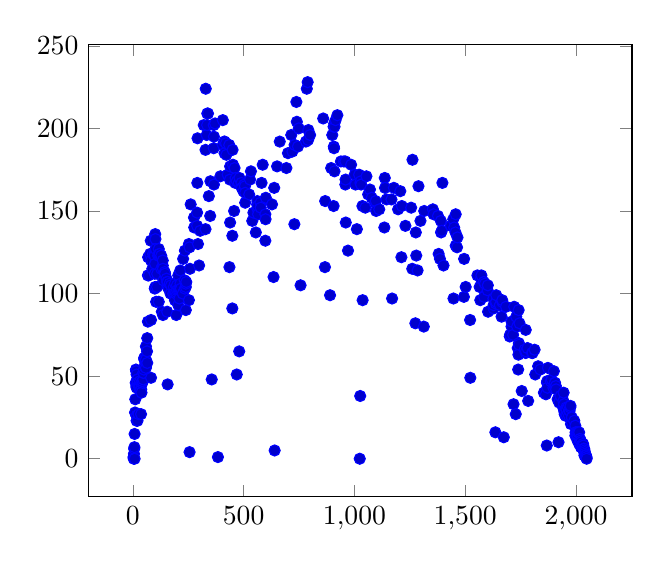
\begin{tikzpicture}
      \begin{axis}[width=0.7\linewidth]
        \addplot+[only marks] coordinates {
          (    3,     1)
          (    4,     0)
          (    5,     3)
          (    6,     6)
          (    7,     7)
          (    8,     0)
          (    8,    15)
          (   10,    28)
          (   11,    36)
          (   13,    46)
          (   14,    54)
          (   15,    53)
          (   16,    44)
          (   17,    23)
          (   17,    26)
          (   17,    43)
          (   17,    51)
          (   18,    26)
          (   20,    48)
          (   21,    23)
          (   21,    48)
          (   22,    46)
          (   26,    27)
          (   26,    44)
          (   27,    45)
          (   28,    44)
          (   29,    44)
          (   31,    42)
          (   32,    42)
          (   33,    44)
          (   33,    47)
          (   36,    42)
          (   37,    27)
          (   38,    42)
          (   38,    46)
          (   39,    40)
          (   43,    46)
          (   43,    47)
          (   44,    47)
          (   47,    48)
          (   47,    52)
          (   48,    52)
          (   50,    54)
          (   51,    61)
          (   52,    60)
          (   53,    56)
          (   58,    58)
          (   59,    55)
          (   59,    60)
          (   59,    68)
          (   64,    65)
          (   65,    58)
          (   65,    73)
          (   68,   111)
          (   68,    83)
          (   69,   122)
          (   72,   111)
          (   78,   124)
          (   81,   132)
          (   82,   120)
          (   82,    49)
          (   82,    84)
          (   88,   115)
          (   91,   124)
          (   97,   124)
          (   98,   123)
          (   99,   103)
          (   99,   112)
          (  100,   118)
          (  101,   104)
          (  101,   136)
          (  102,   133)
          (  103,   127)
          (  105,    95)
          (  109,   104)
          (  110,   112)
          (  114,   123)
          (  117,   127)
          (  117,    95)
          (  119,   123)
          (  119,   124)
          (  120,   123)
          (  121,   124)
          (  128,   115)
          (  128,   123)
          (  131,    89)
          (  135,   117)
          (  135,   120)
          (  136,   115)
          (  136,    87)
          (  138,   108)
          (  144,   113)
          (  145,   112)
          (  152,   109)
          (  155,   107)
          (  155,    89)
          (  156,   107)
          (  157,   104)
          (  157,   107)
          (  157,    45)
          (  162,   103)
          (  166,   106)
          (  170,   100)
          (  172,   105)
          (  182,   100)
          (  185,   104)
          (  187,   100)
          (  190,   106)
          (  190,    96)
          (  194,   100)
          (  196,   101)
          (  196,    87)
          (  199,   105)
          (  200,   102)
          (  205,   111)
          (  205,    93)
          (  206,   102)
          (  210,    97)
          (  211,   102)
          (  214,   114)
          (  215,   106)
          (  216,   102)
          (  217,   103)
          (  225,   100)
          (  227,   121)
          (  234,   108)
          (  235,   103)
          (  235,   126)
          (  239,   104)
          (  239,   106)
          (  239,    90)
          (  241,   107)
          (  253,   130)
          (  253,    96)
          (  256,   128)
          (  256,     4)
          (  258,   115)
          (  261,   154)
          (  276,   146)
          (  277,   140)
          (  290,   141)
          (  290,   149)
          (  291,   167)
          (  292,   194)
          (  294,   130)
          (  299,   117)
          (  304,   138)
          (  320,   202)
          (  328,   139)
          (  328,   187)
          (  329,   224)
          (  333,   196)
          (  335,   202)
          (  336,   209)
          (  339,   209)
          (  343,   159)
          (  349,   147)
          (  350,   168)
          (  356,    48)
          (  365,   188)
          (  365,   202)
          (  366,   166)
          (  366,   195)
          (  371,   203)
          (  384,     1)
          (  395,   171)
          (  406,   190)
          (  406,   205)
          (  413,   192)
          (  414,   185)
          (  414,   192)
          (  420,   191)
          (  422,   184)
          (  428,   172)
          (  435,   190)
          (  436,   116)
          (  438,   169)
          (  439,   143)
          (  439,   177)
          (  449,   135)
          (  449,    91)
          (  450,   187)
          (  452,   178)
          (  457,   150)
          (  459,   176)
          (  462,   167)
          (  464,   170)
          (  469,   168)
          (  469,    51)
          (  478,   167)
          (  480,    65)
          (  481,   170)
          (  489,   165)
          (  490,   167)
          (  492,   164)
          (  499,   162)
          (  503,   166)
          (  506,   165)
          (  507,   155)
          (  507,   161)
          (  525,   160)
          (  529,   169)
          (  533,   174)
          (  539,   144)
          (  544,   149)
          (  555,   137)
          (  561,   154)
          (  562,   156)
          (  563,   151)
          (  564,   153)
          (  565,   148)
          (  576,   155)
          (  577,   152)
          (  581,   167)
          (  586,   178)
          (  598,   132)
          (  598,   148)
          (  599,   145)
          (  600,   158)
          (  628,   154)
          (  635,   110)
          (  638,   164)
          (  640,     5)
          (  651,   177)
          (  663,   192)
          (  693,   176)
          (  700,   185)
          (  715,   196)
          (  720,   186)
          (  729,   142)
          (  730,   190)
          (  738,   216)
          (  740,   204)
          (  745,   189)
          (  749,   200)
          (  757,   105)
          (  781,   192)
          (  785,   224)
          (  789,   228)
          (  791,   193)
          (  792,   199)
          (  800,   196)
          (  859,   206)
          (  867,   116)
          (  868,   156)
          (  890,    99)
          (  895,   176)
          (  900,   196)
          (  906,   153)
          (  906,   201)
          (  907,   189)
          (  908,   188)
          (  909,   203)
          (  910,   174)
          (  910,   201)
          (  915,   205)
          (  923,   208)
          (  939,   180)
          (  952,   180)
          (  959,   166)
          (  959,   180)
          (  960,   169)
          (  961,   143)
          (  971,   126)
          (  985,   178)
          ( 1001,   172)
          ( 1005,   166)
          ( 1011,   139)
          ( 1021,   172)
          ( 1024,     0)
          ( 1026,    38)
          ( 1027,   167)
          ( 1029,   168)
          ( 1030,   166)
          ( 1036,   153)
          ( 1037,    96)
          ( 1049,   152)
          ( 1054,   171)
          ( 1062,   160)
          ( 1070,   163)
          ( 1078,   158)
          ( 1094,   155)
          ( 1096,   156)
          ( 1098,   150)
          ( 1112,   151)
          ( 1135,   140)
          ( 1137,   170)
          ( 1138,   164)
          ( 1145,   157)
          ( 1167,   157)
          ( 1170,    97)
          ( 1178,   164)
          ( 1197,   151)
          ( 1207,   162)
          ( 1212,   122)
          ( 1214,   153)
          ( 1230,   141)
          ( 1256,   152)
          ( 1261,   115)
          ( 1262,   181)
          ( 1275,    82)
          ( 1277,   137)
          ( 1279,   123)
          ( 1285,   114)
          ( 1289,   165)
          ( 1298,   144)
          ( 1313,    80)
          ( 1315,   150)
          ( 1354,   151)
          ( 1357,   148)
          ( 1377,   147)
          ( 1380,   124)
          ( 1386,   121)
          ( 1390,   144)
          ( 1391,   137)
          ( 1394,   138)
          ( 1397,   167)
          ( 1402,   117)
          ( 1435,   141)
          ( 1446,   145)
          ( 1447,    97)
          ( 1450,   140)
          ( 1456,   137)
          ( 1457,   129)
          ( 1457,   148)
          ( 1463,   128)
          ( 1465,   134)
          ( 1494,    98)
          ( 1495,   121)
          ( 1502,   104)
          ( 1522,    84)
          ( 1523,    49)
          ( 1555,   111)
          ( 1565,   104)
          ( 1568,    96)
          ( 1571,   109)
          ( 1573,   111)
          ( 1584,   107)
          ( 1585,    98)
          ( 1589,   106)
          ( 1601,   102)
          ( 1602,   105)
          ( 1603,    89)
          ( 1627,    97)
          ( 1628,    91)
          ( 1628,    93)
          ( 1636,    16)
          ( 1638,    94)
          ( 1639,    95)
          ( 1640,    99)
          ( 1656,    93)
          ( 1664,    86)
          ( 1667,    95)
          ( 1667,    96)
          ( 1674,    13)
          ( 1684,    92)
          ( 1701,    74)
          ( 1702,    75)
          ( 1709,    80)
          ( 1709,    83)
          ( 1716,    75)
          ( 1718,    33)
          ( 1721,    92)
          ( 1728,    27)
          ( 1730,    86)
          ( 1734,    80)
          ( 1737,    67)
          ( 1739,    54)
          ( 1740,    63)
          ( 1741,    90)
          ( 1742,    70)
          ( 1743,    69)
          ( 1745,    82)
          ( 1755,    41)
          ( 1768,    66)
          ( 1773,    64)
          ( 1773,    78)
          ( 1774,    65)
          ( 1781,    67)
          ( 1784,    35)
          ( 1801,    64)
          ( 1804,    64)
          ( 1813,    66)
          ( 1816,    51)
          ( 1829,    56)
          ( 1839,    54)
          ( 1855,    40)
          ( 1864,    39)
          ( 1868,     8)
          ( 1869,    46)
          ( 1870,    47)
          ( 1871,    43)
          ( 1873,    55)
          ( 1886,    47)
          ( 1890,    48)
          ( 1898,    43)
          ( 1900,    53)
          ( 1903,    44)
          ( 1904,    46)
          ( 1905,    46)
          ( 1909,    44)
          ( 1910,    42)
          ( 1917,    36)
          ( 1921,    10)
          ( 1924,    34)
          ( 1930,    38)
          ( 1942,    31)
          ( 1943,    35)
          ( 1944,    40)
          ( 1945,    31)
          ( 1946,    33)
          ( 1947,    29)
          ( 1949,    27)
          ( 1949,    28)
          ( 1953,    26)
          ( 1956,    31)
          ( 1957,    30)
          ( 1959,    26)
          ( 1964,    31)
          ( 1968,    26)
          ( 1971,    29)
          ( 1974,    31)
          ( 1975,    32)
          ( 1977,    21)
          ( 1981,    22)
          ( 1981,    25)
          ( 1992,    23)
          ( 1997,    14)
          ( 1997,    20)
          ( 1998,    16)
          ( 2003,    14)
          ( 2003,    15)
          ( 2004,    16)
          ( 2007,    11)
          ( 2008,    11)
          ( 2008,    14)
          ( 2009,    16)
          ( 2014,    16)
          ( 2014,     9)
          ( 2018,    12)
          ( 2021,    11)
          ( 2022,     7)
          ( 2023,    10)
          ( 2024,     8)
          ( 2028,     7)
          ( 2031,     7)
          ( 2032,     9)
          ( 2033,     8)
          ( 2034,     5)
          ( 2034,     6)
          ( 2035,     5)
          ( 2035,     6)
          ( 2037,     6)
          ( 2038,     2)
          ( 2038,     5)
          ( 2039,     4)
          ( 2040,     3)
          ( 2042,     2)
          ( 2043,     2)
          ( 2044,     1)
          ( 2044,     2)
          ( 2045,     2)
          ( 2046,     1)
          ( 2047,     1)
          ( 2048,     0)
        };
      \end{axis}
    \end{tikzpicture}
  \end{center}
\end{frame}

\begin{frame}[fragile]

  \onslide<+->

  \begin{center}
    \begin{block}{Code}
      \begin{lstlisting}
(def points
     (map (fn [_]
            (let [ctx (reduce-context (random-context (rand-int 2048)
                                                      11
                                                      (rand)))]
              (list (count (intents ctx))
                    (count (pseudo-intents ctx)))))
          (range 1 1000)))
      \end{lstlisting}
    \end{block}
  \end{center}

\end{frame}

\subsection{In Case You Need Help}

\begin{frame}

  \onslide<+->

  \begin{code}{}
    \codeio{(doc make-context)}{------------------------\\
      conexp.main/make-context\\
      ([objects attributes incidence])\\
      \ \ Standard constructor for contexts. Takes a sequence of objects,\\
      \ \ a sequence of attributes and either a set of pairs or function of\\
      ...\\
      nil}
    \codeio{(find-doc "formal context")}{------------------------\\
      conexp.fca.implications/proper-premises-by-hypertrans\\
      ...\\
      conexp.fca.implications/proper-premises-for-attribute\\
      ...
    }
  \end{code}  
\end{frame}

\section{The End}

\subsection{Outlook and Further Development}

\begin{frame}
  \onslide<+->
  \begin{block}{The Future}
    \begin{itemize}
    \item<+-> A better GUI
    \item<+-> Java backend for more performance
    \item<+-> More flexible IO system
    \item<+-> More documentation
    \end{itemize}
  \end{block}
  \onslide<+->
  \begin{block}{Alternate Reality}
    \begin{itemize}
    \item<+-> Reimplementation in Guile (Scheme, Python, Lua, ...)
    \item<+-> C backend for better performance
    \item<+-> Retain flexibility, but increase speed
    \end{itemize}
  \end{block}
\end{frame}

\begin{frame}
  \centerline{Exercises!}
\end{frame}

\begin{frame}
  \centerline{Thank You!}
\end{frame}

\end{document}

%%% Local Variables: 
%%% mode: latex
%%% TeX-master: t
%%% TeX-engine: default
%%% ispell-local-dictionary: "american"
%%% End: 
